% -*- latex -*-

\chapter{Execution Environment}
\label{chap:ExecutionEnvironment}

The execution environment is exposed to developers that write worklets for
different visualization algorithms. In addition to providing all the
mechanisms for building the worklet object itself, the execution
environment contains supporting code that can be useful to the
implementations of visualization algorithms.

The data structures in the execution environment provide information and
operations for a single element. This is in contrast to the control
environment, where data structures are built on arrays providing
information for large collections of data. These respective data structures
reflect the nature of the two environments. The control environment manages
the stores of data whereas the execution environment performs large
parallel processing through fine operations.

\section{Creating Worklets}

\index{worklet|(}
\index{worklet!creating|(}

A worklet in VTK-m is most simply a functor that operates on an element of
data. Thus, it is a \textcode{class} or \textcode{struct} that has an
overloaded parenthesis operator (which must be declared \textcode{const}
for thread safety). It also must inherit from one of the predefined
abstract worklet classes, which will declare the correct dispatcher to use
when invoking the worklet. Finally, it must declare a pair of
\index{signature}\keyterm{signatures} that define what information must be
presented when invoking the worklet and how this information gets passed to
each worklet invocation. Figure~\ref{fig:WorkletExampleAnnotated}
demonstrates all of the required components of a worklet.

%% \pagebreak
%% \begin{vtkmexample}{Example Code for Cutting/Pasting.}
%% class TriangulateCell : public vtkm::worklet::WorkletMapPointToCell
%% {
%% public:
%%   typedef void ControlSignature(TopologyIn topology,
%%                                 ExecObject tables,
%%                                 FieldOutCell<> connectivityOut);
%%   typedef void ExecutionSignature(CellShape, PointIndices, _2, _3, VisitIndex);
%%   typedef _1 InputDomain;

%%   typedef vtkm::worklet::ScatterCounting ScatterType;
%%   VTKM_CONT_EXPORT
%%   ScatterType GetScatter() const
%%   {
%%     return this->Scatter;
%%   }

%%   template<typename CellShapeTag,
%%            typename ConnectivityInVec,
%%            typename ConnectivityOutVec>
%%   VTKM_EXEC_EXPORT
%%   void operator()(
%%       CellShapeTag shape,
%%       const ConnectivityInVec &connectivityIn,
%%       const internal::TriangulateTablesExecutionObject<DeviceAdapter> &tables,
%%       ConnectivityOutVec &connectivityOut,
%%       vtkm::IdComponent visitIndex) const
%%   {
%% \end{vtkmexample}
%% \pagebreak

\begin{figure}[htb]
  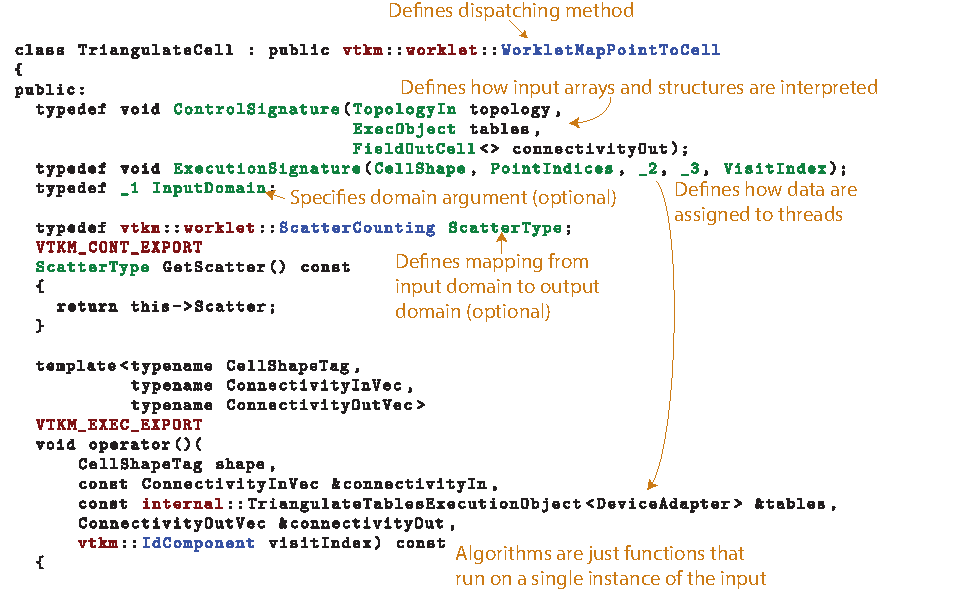
\includegraphics[width=\linewidth]{images/WorkletExampleAnnotated}
  \caption{Annotated example of a worklet declaration.}
  \label{fig:WorkletExampleAnnotated}
\end{figure}

\subsection{Control Signature}
\label{sec:ControlSignature}

\index{control~signature|(}
\index{signature!control|(}
\index{worklet!control~signature|(}

The control signature of a worklet is the \textcode{typedef} of a function
prototype named \controlsignature. The function prototype matches the
calling specification used with the dispatcher invoke function.

The return type of the function prototype is always \textcode{void} because
the dispatcher invoke functions do not return values. The parameters of the
function prototype are \index{signature~tags}\keyterm{tags} that identify
the type of data that is expected to be passed to invoke. For example, a
\sigtag{FieldIn} tag declares that the worklet will operate on input field
data, typically held in a \vtkmcont{ArrayHandle} whereas a
\sigtag{TopologyIn} tag declares that the worklet will operate on a cell set
structure like those documented in Section~\ref{sec:DataSets:CellSets}.

Tags can also have modifiers on them, which are attached as template
parameters. For example, a \sigtag{FieldIn} tag has a template parameter
that allows you to specify what data types can be in the field. A
\sigtagmod{FieldIn}{Scalar} accepts only scalar values whereas
\sigtagmod{FieldIn}{Vec3} accepts only 3D vectors.

The signature tags and their modifiers are described in greater detail in
the following section on worklet types.

\index{worklet!control~signature|)}
\index{signature!control|)}
\index{control~signature|)}

\subsection{Execution Signature}
\label{sec:ExecutionSignature}

\index{execution~signature|(}
\index{signature!execution|(}
\index{worklet!execution~signature|(}

Like the control signature, the execution signature of a worklet is the
\textcode{typedef} of a function prototype named \executionsignature. The
function prototype must match the parenthesis operator in terms of arity
and argument semantics.

The arguments of the \executionsignature's function prototype are tags that
define where the data come from. The most common tags are an underscore
followed by a number, such as \sigtagnum{1}, \sigtagnum{2}, etc. These
numbers refer back to the corresponding argument in the
\controlsignature. For example, \sigtagnum{1} means data from the first
control signature argument, \sigtagnum{2} means data from the second
control signature argument, etc.

Unlike the control signature, the execution signature optionally can
declare a return type if the parenthesis operator returns a value. If this
is the case, the return value should be one of the numeric tags
(i.e. \sigtagnum{1}, \sigtagnum{2}, etc.) to refer to one of the data
structures of the control signature. If the parenthesis operator does not
return a value, then \executionsignature should declare the return type as
\textcode{void}.

In addition to the numeric tags, there are other execution signature tags
to represent other types of data. For example, the \sigtag{WorkIndex} tag
identifies the instance of the worklet invocation. Each call to the worklet
function will have a unique \sigtag{WorkIndex}. Other such tags exist and
are described in the following section on worklet types where appropriate.

\index{worklet!execution~signature|)}
\index{signature!execution|)}
\index{execution~signature|)}

\subsection{Input Domain}
\label{sec:InputDomain}

\index{input~domain|(}
\index{worklet!input~domain|(}

Every worklet has one input argument in the \controlsignature identified as
its input domain. When a dispatcher invokes a worklet, it uses the input
argument to determine how many instances of the worklet to run.

Different types of worklets can have different types of domain. For example
a simple field map worklet has a \sigtag{FieldIn} argument as its input
domain, and the size of the input domain is taken from the size of the
associated field array. Likewise, a worklet that maps topology has a
\sigtag{TopologyIn} argument as its input domain, and the size of the input
domain is taken from the cell set.

A worklet specifies its input domain by creating a \textcode{typedef} named
\sigtag{InputDomain}. The object used in the \textcode{typedef} should be
one of the numeric tags (i.e. \sigtagnum{1}, \sigtagnum{2}, etc.) that
points to the appropriate \controlsignature argument.

Specifying the \sigtag{InputDomain} is optional. If it is not specified,
the first argument is assumed to be the input domain.

\index{worklet!input~domain|)}
\index{input~domain|)}

\subsection{Scatter}
\label{sec:WorkletScatter}

\index{scatter|(}
\index{worklet!scatter|(}

\fix{Don't forget scatters.}

\index{worklet!scatter|)}
\index{scatter|)}

\index{worklet!creating|)}
\index{worklet|)}

\section{Error Handling}
\label{sec:ExecutionEnvironment:ErrorHandling}

\section{Math}


\section{Working with Topology}

In the control environment, data is defined in mesh structures that
comprise a set of finite cells. (See Section~\ref{sec:DataSets:CellSets}
starting on page~\pageref{sec:DataSets:CellSets} for information on
defining cell sets in the control environment.) When worklets that operate
on cells are scheduled, these grid structures are broken into their
independent cells, and that data is handed to the worklet. Thus, cell-based
operations in the execution environment exclusively operate on independent
cells.

Unlike some other libraries such as VTK, VTK-m does not have a cell class
that holds all the information pertaining to a cell of a particular type.
Instead, VTK-m provides tags or identifiers defining the cell shape, and
companion data like coordinate and field information are held in separate
structures. This organization is designed so a worklet may specify exactly
what information it needs, and only that information will be loaded.

\subsection{Cell Shape Tags and Ids}
\label{sec:CellShapeTagsIds}

\index{shape|(}
\index{cell~shape|(}
\index{tag!cell~shape|(}
\index{tag!shape|(}

Cell shapes can be specified with either a tag (defined with a struct with
a name like \textidentifier{CellShapeTag*}) or an enumerated identifier
(defined with a constant number with a name like
\textidentifier{CELL\_SHAPE\_*}). These shape tags and identifiers are
defined in \vtkmheader{vtkm}{CellShape.h} and declared in the \vtkm{}
namespace (because they can be used in either the control or the execution
environment). Figure~\ref{fig:CellShapes} gives both the identifier and the
tag names.

\begin{figure}
  \centering
  \small
  \begin{tabular}{@{}c@{~}c@{~}c@{}}
    \raisebox{-0.5\height}{
\includegraphics{images/CellConnectionsVertex}} &
    \raisebox{-0.5\height}{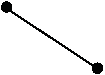
\includegraphics{images/CellConnectionsLine}} &
    \raisebox{-0.5\height}{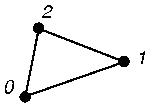
\includegraphics{images/CellConnectionsTriangle}} \\
    \vtkm{CELL\_SHAPE\_VERTEX} &
    \vtkm{CELL\_SHAPE\_LINE} &
    \vtkm{CELL\_SHAPE\_TRIANGLE} \\
    \vtkm{CellShapeTagVertex} \index{vertex} &
    \vtkm{CellShapeTagLine} \index{line} &
    \vtkm{CellShapeTagTriangle} \index{triangle} \\[2ex]
    \raisebox{-0.5\height}{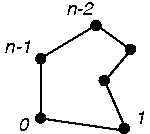
\includegraphics{images/CellConnectionsPolygon}} &
    \raisebox{-0.5\height}{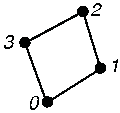
\includegraphics{images/CellConnectionsQuadrilateral}} &
    \raisebox{-0.5\height}{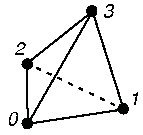
\includegraphics{images/CellConnectionsTetrahedron}} \\
    \vtkm{CELL\_SHAPE\_POLYGON} &
    \vtkm{CELL\_SHAPE\_QUAD} &
    \vtkm{CELL\_SHAPE\_TETRA} \\
    \vtkm{CellShapeTagPolygon} \index{polygon} &
    \vtkm{CellShapeTagQuad} \index{quadrilateral} &
    \vtkm{CellShapeTagTetra} \index{tetrahedron} \\[2ex]
    \raisebox{-0.5\height}{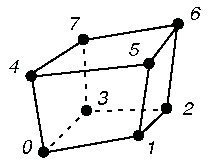
\includegraphics{images/CellConnectionsHexahedron}} &
    \raisebox{-0.5\height}{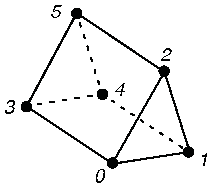
\includegraphics{images/CellConnectionsWedge}} &
    \raisebox{-0.5\height}{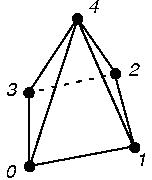
\includegraphics{images/CellConnectionsPyramid}} \\
    \vtkm{CELL\_SHAPE\_HEXAHEDRON} &
    \vtkm{CELL\_SHAPE\_WEDGE} &
    \vtkm{CELL\_SHAPE\_PYRAMID} \\
    \vtkm{CellShapeTagHexahedron} \index{hexahedron} &
    \vtkm{CellShapeTagWedge} \index{wedge} &
    \vtkm{CellShapeTagPyramid} \index{pyramid}
  \end{tabular}
  \caption{Basic Cell Shapes}
  \label{fig:CellShapes}
\end{figure}

In addition to the basic cell shapes, there is a special ``empty'' cell
with the identifier \vtkm{CELL\_SHAPE\_EMPTY} and tag
\vtkm{CellShapeTagEmpty}. This type of cell has no points, edges, or faces
and can be thought of as a placeholder for a null or void cell.

There is also a special cell shape ``tag'' named \vtkm{CellShapeTagGeneric}
that is used when the actual cell shape is not known at compile time.
\textidentifier{CellShapeTagGeneric} actually has a member variable named
\textcode{Id} that stores the identifier for the cell shape. There is no
equivalent identifier for a generic cell; cell shape identifiers can be
placed in a \vtkm{IdComponent} at runtime.

\fix{Add other basic cell shape features such as traits, converting back
  and forth, and \vtkmmacro{vtkmGenericCellShapeMacro}.}

\index{tag!shape|)}
\index{tag!cell~shape|)}
\index{cell~shape|)}
\index{shape|)}

\subsection{Parametric and World Coordinates}

\subsection{Interpolation}

\subsection{Derivatives}
